\documentclass[12pt, spanish]{article}
\usepackage[spanish]{babel}
\selectlanguage{spanish}
\usepackage{natbib}
\usepackage{url}
\usepackage[utf8x]{inputenc}
\usepackage{graphicx}
\graphicspath{{images/}}
\usepackage{parskip}
\usepackage{fancyhdr}
\usepackage{vmargin}


\usepackage{tikz}
\usepackage{amsfonts}


\usepackage{hyperref}
\usepackage[
    type={CC},
    modifier={by-nc-sa},
    version={4.0},
]{doclicense}

\hypersetup{
    colorlinks=true,
    linkcolor=blue,
    filecolor=magenta,      
    urlcolor=cyan,
}

\usepackage[default]{sourcesanspro}

\setmarginsrb{2 cm}{1 cm}{2 cm}{2 cm}{1 cm}{1.5 cm}{1 cm}{1.5 cm}

\title{Modelos de Computación:\\
Ejercicios. \hspace{0.05cm} }                           
\author{Antonio David Villegas Yeguas}                             
\date{\today}                                           

\renewcommand*\contentsname{hola}

\makeatletter
\let\thetitle\@title
\let\theauthor\@author
\let\thedate\@date
\makeatother

\pagestyle{fancy}
\fancyhf{}
\rhead{\theauthor}
\lhead{\thetitle}
\cfoot{\thepage}

\begin{document}
%%%%%%%%%%%%%%%%%%%%%%%%%%%%%%%%%%%%%%%%%%%%%%%%%%%%%%%%%%%%%%%%%%%%%%%%%%%%%%%%%%%%%%%%%

\begin{titlepage}
    \centering
    \vspace*{0.5 cm}
    
\includegraphics[scale = 0.50]{ugr.png}\\[1.0 cm]
    %\textsc{\LARGE Universidad de Granada}\\[2.0 cm]   
    \textsc{\large 3ºA - A2}\\[0.5 cm]            
    \textsc{\large Grado en Ingeniería Informática}\\[0.5 cm]              
    \rule{\linewidth}{0.2 mm} \\[0.2 cm]
    { \huge \bfseries \thetitle}\\
    \rule{\linewidth}{0.2 mm} \\[1 cm]
    
    \begin{minipage}{0.4\textwidth}
        \begin{flushleft} \large
            \emph{Autor:}\\
            \theauthor
            \end{flushleft}
            \end{minipage}~
            \begin{minipage}{0.4\textwidth}
            \begin{flushright} \large
            \emph{Asignatura: \\
            Modelos de Computación}                   
        \end{flushright}
    \end{minipage}\\[0.5cm]
  
    {\large \thedate}\\[0.5cm]
    {\url{https://github.com/advy99/MC/}}
    {\doclicenseThis}
 	
    \vfill
    
\end{titlepage}

%%%%%%%%%%%%%%%%%%%%%%%%%%%%%%%%%%%%%%%%%%%%%%%%%%%%%%%%%%%%%%%%%%%%%%%%%%%%%%%%%%%%%%%%%

%\tableofcontents
%\pagebreak

%%%%%%%%%%%%%%%%%%%%%%%%%%%%%%%%%%%%%%%%%%%%%%%%%%%%%%%%%%%%%%%%%%%%%%%%%%%%%%%%%%%%%%%%%

\section{Ejercicio 1:} 

Determinar si G = ({S, A, B}, {a, b, c, d}, P, S) donde P es el conjunto de reglas de producción:

$$ S \rightarrow AB $$
$$ A \rightarrow Ab | a $$
$$ B \rightarrow cB | d $$

Genera un lenguaje de tipo 3.

\textbf{Respuesta:}

Vemos como esta gramática genera el siguiente lenguaje:

$$ L = \{ab^ic^jd / i, j \in \mathbb{N} / i, j \geq 0\} $$

Vemos como esto sigue una forma regular, ya que podemos generar este lenguaje de izquierda a derecha ya que no tenemos dependencias entre unos símbolos terminales y otros. Podemos generar este lenguaje a partir de la siguiente gramática:

$$ S \rightarrow aB $$
$$ B \rightarrow bB | C $$
$$ C \rightarrow cC | d $$

En la primera regla generamos la a obligatoria y pasamos a generar b's, en la regla B generamos una ristra de b's y pasamos a generar c's, aunque podemos pasar directamente a generar c's sin generar b's, cumpliendo que $i \geq 0$, en C generamos una ristra de c's o una d, aunque podríamos no generar ninguna c, cumpliendo $j \geq 0$, pero la d si es obligatoria.

Como esta gramática es de tipo 3, L es de tipo 3.

\newpage

\section{Ejercicio 2:}

Construir una máquina de estados que calcule el complemento a 2 de un número en binario.

\textbf{Respuesta:}

El complemento a 2 se basa en realizar el complemento a 1 en un número en binario y después sumarle 1.

Primero crearemos la máquina para calcular el complemento a 1, que se basa en cambiar 0's por 1's. Por este motivo voy a escoger una máquina de Mealy, ya que la salida depende de la entrada.


\begin{center}
	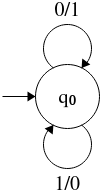
\includegraphics[scale=0.7]{maquina_1.png}
\end{center}

Una vez tenemos la máquina de Mealy capaz de crear complemento a 1, pasamos a calcular el complemento a 2.

\begin{table}[h]
\begin{tabular}{lllllllllll}
                &  & 0 & 0 & 1 & 1 & 0 & 1 & 0 & 0 & 0  \\
Complemento a 1 &  &   &   &   &   &   &   &   &   &    \\ \hline
                &  & 1 & 1 & 0 & 0 & 1 & 0 & 1 & 1 & 1  \\
Complemento a 2 &  &   &   &   &   &   &   &   & +  & 1 \\ \hline
                &  & 1 & 1 & 0 & 0 & 1 & 1 & 0 & 0 & 0 
\end{tabular}
\end{table}


Vemos como el complemento a 2 es exactamente igual que la cadena introducida hasta que encontramos el primer 1. El primer 1 se sigue manteniendo y a partir de ahí la cadena pasa a ser el complemento a 1 de la original.

El hacer nuestra máquina de esta forma también implica que leerá de derecha a izquierda, y no de izquierda a derecha.

Como la salida depende de la entrada, volvemos a escoger la máquina de Mealy.

\newpage

El resultado será el siguiente:

\begin{center}
	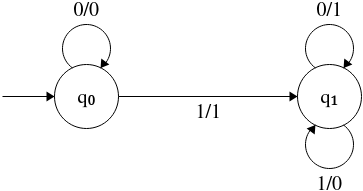
\includegraphics[scale=0.7]{maquina_2.png}
\end{center}


En el estado $q_0$ mantenemos los 0's iniciales, hasta encontrar el primer 1, que también mantenemos pero pasamos al estado $q_1$, en este estado cambiamos los 0's por 1's y viceversa.




\section{Ejercicio 3:}

Si es posible, construir un AFD para el siguiente lenguaje:

$$ L = \{ pcp^{-1} / p \in \{0, 1\}^* \} $$

En caso contrario demostrar que no existe dicho AFD

\textbf{Respuesta:}

Vemos como el lenguaje no es regular ya que presenta dependencias entre distintas partes separadas de sus cadenas, luego usaremos el lema de bombeo para demostrar que no es regular y que no existe dicho AFD.

El lema de bombeo dicta lo siguiente:

Sea L un conjunto regular, entonces $\exists n \in \mathbb{N}$ tal que $\forall z \in $, si $|z| \geq n$, entonces z se puede expresar de la forma z = uvw donde:

\begin{enumerate}
	\item $|uv| \leq n$
	\item $|v| \geq 1$
	\item $(\forall i \geq 0) uv^iw \in L$
\end{enumerate} 


Por lo que para comprobar si un lenguaje no es regular, negaremos el lema de bombeo sobre el lenguaje L:

Sea L un conjunto regular, entonces $\forall n \in \mathbb{N}$ tal que $\exists z \in L$, si $|z| \geq n$, entonces $\forall z = uvw$ donde:


\begin{enumerate}
	\item $|uv| \leq n$
	\item $|v| \geq 1$
	\item $(\exists i \geq 0) uv^iw \not \in L$
\end{enumerate}



Primero, para cualquier n tenemos que escoger una palabra z que pertenezca al lenguaje. Yo escogeré la siguiente palabra: $z = 0^nc0^n$. Como vemos trivialmente, esta palabra esta dentro del lenguaje.


Por el lema de bombeo, podemos descomponer z en:

\begin{enumerate}
	\item $u = 0^k$
	\item $v = 0^l$
	\item $w =0^{n-l-k}c0^n$
\end{enumerate}

Siguiendo el lema de bombeo, existe una i tal que:

$$ uv^iw \not \in L $$
$$uv^iw = 0^k0^{li}0^{n-l-k}c0^n = $$
$$ = 0^{n + li - l + k - k}c0^n  = $$
$$ = 0^{n + l(i - 1)}c0^n  $$

Vemos como si $i = 2$

$$ uv^iw = 0^{n+l}c0^n $$

Como sabemos que $l \geq 1$, entonces $ n + l > n $ luego la parte izquierda de c tienes más ceros que la derecha, y no pueden ser palíndromos, luego 

$$ uv^2w \not \in L $$

Así que hemos demostrado que L no es regular y por lo tanto no existe un AFD para este lenguaje.


\newpage


\section{Ejercicio 4:}

Construir un autómata con pila para aceptar palíndromos de 0's y 1's.

$$ L = \{ u \in \{0, 1\}^* / u = u^{-1} \} $$

\textbf{Respuesta:}

\begin{center}
	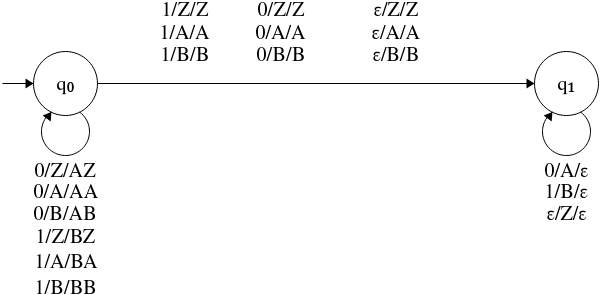
\includegraphics[scale=0.5]{aut_pila.png}
\end{center}

Para resolver este problema creamos un autómata con pila que aceptará cadenas por el criterio de pila vacía.

Este autómata tendrá dos estados, $q_0$ y $q_1$. Además, la pila podrá tener los símbolos Z (símbolo inicial), A (hemos leído un 0) y B (hemos leído un 1).

En $q_0$ añadiremos elementos en la pila para almacenar que caracteres hemos introducido, teniendo en cuenta todos los casos posibles (tanto para un 0 o un 1, que en el tope de pila este el símbolo inicial Z, el símbolo A, o el símbolo B).

En $q_1$ desapilamos los distintos símbolos de la pila, aunque solo un 0 puede quitar de la pila una A, solo un 1 puede quitar una B, y solo cuando nos quedemos sin palabra quitaremos la Z. Este paso lo hacemos para comprobar que la segunda parte de la cadena es igual que la primera. Si por ejemplo leemos un 1 y el tope de la pila es una A, es que la cadena no es un palíndromo y no podrá seguir leyendo, luego no aceptará la cadena.

En la transición de $q_0$ a $q_1$ leeremos el símbolo que esta en mitad de la palabra (si el palíndromo es impar) sin modificar la pila, aunque también podemos cambiar de estado sin leer nada ($\epsilon$) para aceptar palíndromos pares.

\end{document}

